\section{System Model and Problem Formulation}
\label{sec:system_model}

\subsection{Environment, Measurements, and Fingerprint}

Consider an indoor area $\mathcal{A}\subset\mathbb{R}^{2}$ with $M$ fixed Wi-Fi access points (APs) at positions $\mathbf{p}_{m}=[x^{\mathrm{AP}}_{m},y^{\mathrm{AP}}_{m}]^{T}$, $m=1,\ldots,M$, and a mobile device at the unknown position $\mathbf{u}=[x,y]^{T}\in\mathcal{A}$. As illustrated in Fig.~\ref{fig:system_model}, the device obtains from each detectable AP an RTT measurement and an RSS measurement,
\begin{align}
	r^{\mathrm{RTT}}_{m} &= h^{\mathrm{RTT}}(\mathbf{u},\mathbf{p}_{m})+\varepsilon^{\mathrm{RTT}}_{m},\\
	r^{\mathrm{RSS}}_{m} &= h^{\mathrm{RSS}}(\mathbf{u},\mathbf{p}_{m},\mathcal{E})+\varepsilon^{\mathrm{RSS}}_{m},
\end{align}
where $h^{\mathrm{RTT}}$ relates the user--AP geometry to the measured round-trip time, $h^{\mathrm{RSS}}$ additionally depends on the propagation environment $\mathcal{E}$, and the error terms capture multipath, NLOS bias, hardware effects, and short-term fluctuations. RTT carries the stronger geometric information, but is biased under NLOS conditions; RSS provides no direct distance but complementary information about the radio environment~\cite{martinescalona2023ftm,eberechukwu2023fusion,dong2023rtt_rss,feng2026robust}.

\begin{figure*}[!t]
	\centering
	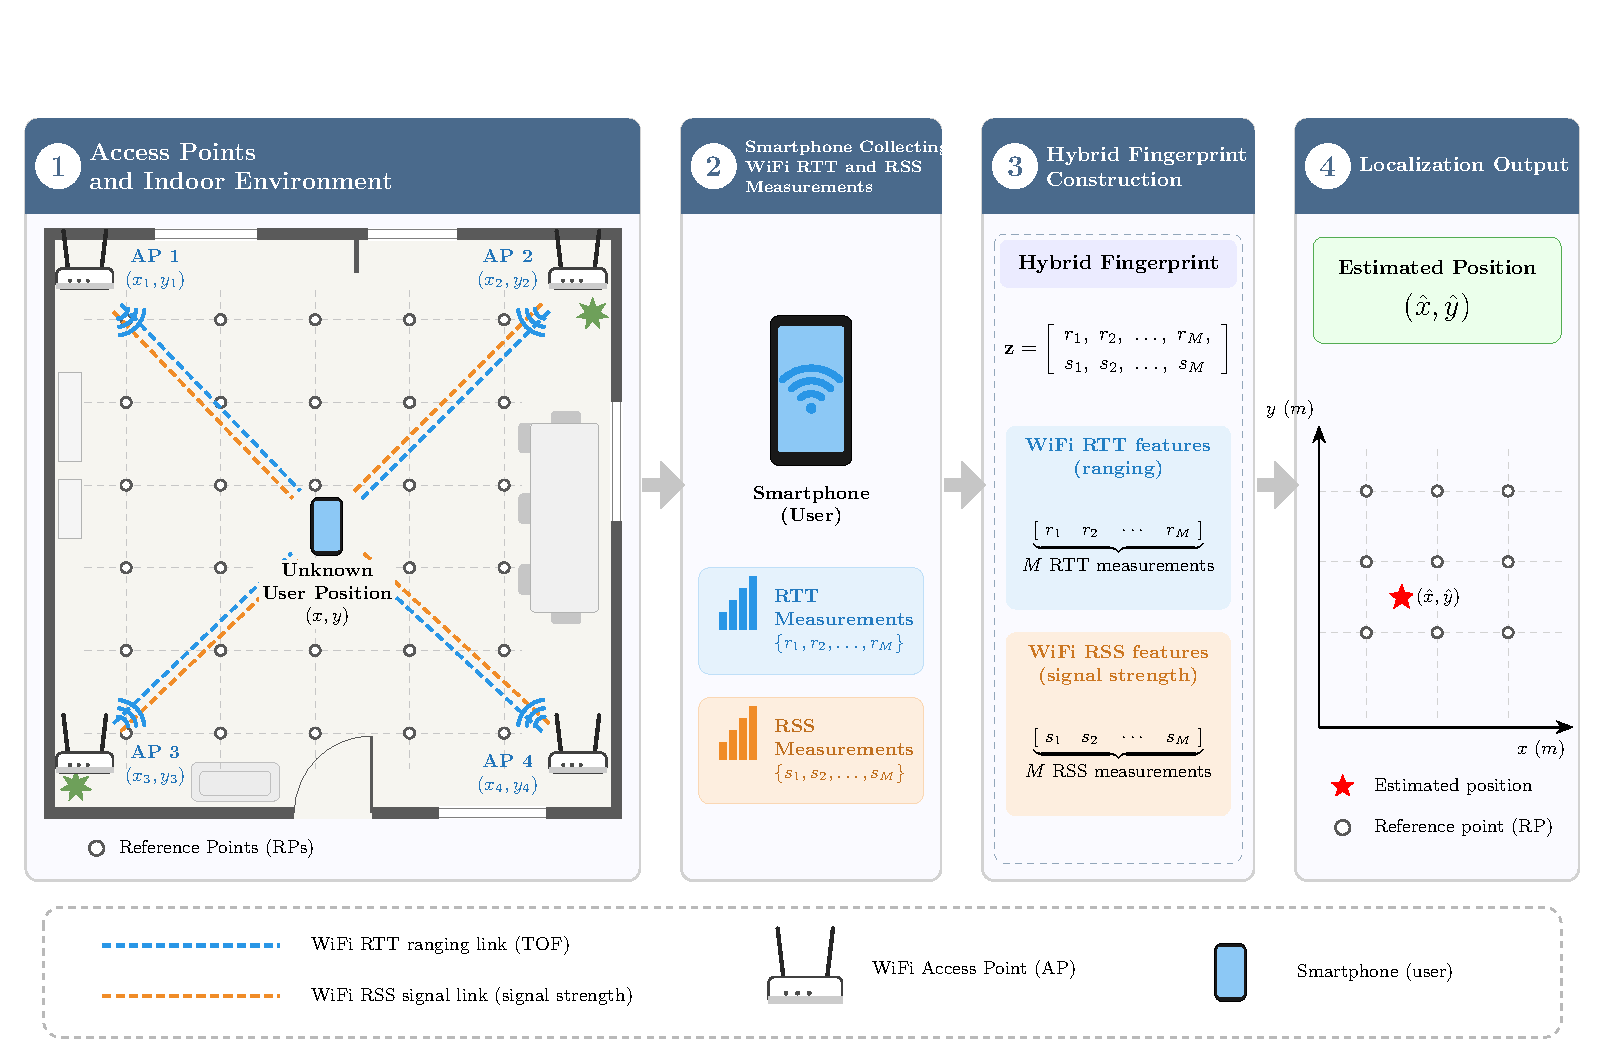
\includegraphics[width=\textwidth]{figures/methodology/fig01_system_model.pdf}
	\caption{System model of the hybrid Wi-Fi RTT--RSS indoor positioning system. A mobile device collects RTT ranging and RSS measurements from surrounding Wi-Fi access points. The measurements are concatenated into a hybrid fingerprint and mapped by the learned positioning model to an estimated two-dimensional user position.}
	\label{fig:system_model}
\end{figure*}

Rather than imposing an explicit propagation model, we follow a fingerprinting formulation. The measurements of one scan form the hybrid fingerprint
\begin{equation}
	\mathbf{z}
	=
	[r^{\mathrm{RTT}}_{1},\ldots,r^{\mathrm{RTT}}_{M},\,r^{\mathrm{RSS}}_{1},\ldots,r^{\mathrm{RSS}}_{M}]^{T}
	\in\mathbb{R}^{p},
	\label{eq:hybrid_fingerprint}
\end{equation}
with $p=2M$ features. APs that are not heard in a scan are encoded with the sentinel value of the respective dataset; no artificial distance is imputed.

\subsection{Fingerprint Database and Reference-Point Groups}

During the offline phase, scans are collected at $N_{\mathrm{RP}}$ known reference points (RPs). The database $\mathcal{D}=\{(\mathbf{z}_{i},\mathbf{u}_{i},g_i)\}_{i=1}^{N}$ contains $N\gg N_{\mathrm{RP}}$ scans with known positions $\mathbf{u}_{i}=[x_i,y_i]^{T}$ and RP identifiers
\begin{equation}
	g_i=g_j
	\quad\Longleftrightarrow\quad
	(x_i,y_i)=(x_j,y_j).
	\label{eq:rp_group}
\end{equation}
In the datasets used here, each RP contributes 100--120 scans per acquisition session. A regression function $f:\mathbb{R}^{p}\rightarrow\mathbb{R}^{2}$, $\hat{\mathbf{u}}=f(\mathbf{z})$, is learned from $\mathcal{D}$.

The grouping defines two evaluation questions. In \emph{sample-level} evaluation, scans of the same RP can appear in training and test data, so the model is asked to recognize new scans at already-surveyed locations. In \emph{RP-disjoint} evaluation, $\mathcal{G}_{\mathrm{train}}\cap\mathcal{G}_{\mathrm{test}}=\varnothing$, so the model must estimate positions at unsurveyed locations. Both are reported in this work, but never mixed.

\subsection{Localization Metrics}
\label{subsec:metrics}

For a test set of $N_t$ scans, the Euclidean error of scan $i$ is $e_i=\|\mathbf{u}_{i}-\hat{\mathbf{u}}_{i}\|_{2}$, with positions expressed in metres (for Dataset~I, grid coordinates are multiplied by the grid spacing $\Delta$ first), and the true two-dimensional RMSE is
\begin{equation}
	\mathrm{RMSE}_{2D}
	=
	\sqrt{\frac{1}{N_t}\sum_{i=1}^{N_t}e_i^{2}}.
	\label{eq:rmse2d}
\end{equation}
We also report the mean error and the $50$th, $90$th, and $95$th percentiles $P_{50}$, $P_{90}$, and $P_{95}$ of $e_i$, because an improvement of the average does not imply an improvement of the tail.

For comparison with the published hybrid RTT--RSS baseline~\cite{feng2026robust}, we additionally report the \emph{paper-compatible} metric
\begin{equation}
	E_{\mathrm{paper}}
	=
	\frac{\mathrm{RMSE}_{x}+\mathrm{RMSE}_{y}}{2}\,\Delta,
	\label{eq:paper_metric}
\end{equation}
where
\begin{align}
	\mathrm{RMSE}_{x}&=\sqrt{\frac{1}{N_t}\sum_{i=1}^{N_t}(x_i-\hat{x}_i)^{2}},\\
	\mathrm{RMSE}_{y}&=\sqrt{\frac{1}{N_t}\sum_{i=1}^{N_t}(y_i-\hat{y}_i)^{2}},
\end{align}
and $\Delta$ is the grid spacing that converts the dataset's coordinate units into metres. Because it averages per-coordinate errors, $E_{\mathrm{paper}}$ is about $\sqrt{2}$ times smaller than $\mathrm{RMSE}_{2D}$ for isotropic errors; the two are never treated as interchangeable.

\subsection{Problem Statement}

Given $\mathcal{D}$, the objective is a positioning model that (i) minimizes the localization error at unsurveyed locations, (ii) remains cheap to train and to evaluate online, (iii) is configured and validated without leakage between scans of the same RP, and (iv) optionally returns a region $\mathcal{C}_{1-\alpha}(\mathbf{z})\subset\mathbb{R}^{2}$ that contains the true position with probability at least $1-\alpha$. Section~\ref{sec:proposed_method} addresses (i)--(iii) through the subspace ratio of a Random Forest and (iv) through conformal calibration.
